\documentclass[10pt, conference, compsocconf]{IEEEtran}

\usepackage[english]{babel}
\usepackage{latexsym}
\usepackage{amssymb}
\usepackage{graphicx}
\usepackage{multirow}
\usepackage{url}
\usepackage{subfig}
\usepackage{ifthen}
\usepackage{listings}
\usepackage{graphvizzz}
\usepackage{minted}

% Very convenient to add comments on the paper. Just set the boolean
% to false before sending the paper:
\newboolean{showcomments}
\setboolean{showcomments}{true}
\ifthenelse{\boolean{showcomments}}
{ \newcommand{\mynote}[2]{
    \fbox{\bfseries\sffamily\scriptsize#1}
    {\small$\blacktriangleright$\textsf{\emph{#2}}$\blacktriangleleft$}}}
{ \newcommand{\mynote}[2]{}}

% One command per author:
\newcommand{\cd}[1]{\mynote{Corentin}{#1}}
\newcommand{\ms}[1]{\mynote{Mehdi}{#1}}
\newcommand{\ff}[1]{\mynote{Fede}{#1}}
\newcommand{\todo}[1]{\mynote{Todo}{#1}}

\DeclareCaptionType{copyrightbox}
%\setlength{\belowcaptionskip}{-10pt}
%\setlength{\abovecaptionskip}{-10pt}
\setlength\partopsep{-\topsep}

\begin{document}

\title{Optimized PaaS Architectures: Qualifying the Flexibility of Applications}

\author{\IEEEauthorblockN{Corentin Dupont, Mehdi Sheikhalishahi, Federico Facca}
\IEEEauthorblockA{Create-Net\\
Trento, Italy\\
\{cdupont, msheikhalishahi, ffacca\}@create-net.org
}
}

\maketitle
\begin{abstract}
% !TEX root =  main.tex


Data centres are power-hungry facilities that hosts ICT services and consumes up consume up to 3\% of all global electricity production.
Consequently, in the last years, trend research in the field focused on mechanisms reduce the overall consumption of a data centre so as to reduce its energy footprint.
Following such research outcomes, several data centre management frameworks started to implement energy efficiency policies.
Such energy management techniques - with the help of other factors,  such as introduction of less power greedy CPUs - had a positive impact: a recent study showed that the energy consumption of data centres is actually less than the one previously predicted.
However, from a research perspective, techniques for reducing energy consumption of virtualized infrastructures - such as server consolidation - are now well-known and not great breakthrough are expected.
The introduction of new solutions - such as containers and platform as a service - in cloud data-centers open new challenges and opportunities.
Moreover the new interest toward aspects such as green footprint, demand for more than just reducing energy consumption. 
Aiming at reducing energy consumption in data centres becomes part of a larger equation: being able to consume energy in a better way, prioritizing the consumption of green energies.
In this paper we present the concept of Service Flexibility Agreement (SFA), an extension of the traditional SLA able to qualify the flexibility of applications deployed in a cloud environment. The concept is exploited to manage applications according to a given power budget. In particular, we detail preliminary models able to exploit this flexibility in order to increase the ratio of renewable energy consumed, notably in the case of local production (e.g. solar panels).
Finally, we describe how the combination of PaaS and IaaS cloud layers provide the needed flexibility to support the SFA.

\end{abstract}

\begin{IEEEkeywords}
Platform as a Service, Energy Management, Flexibility, Scalability
\end{IEEEkeywords}

% !TEX root =  main.tex
\section{Introduction}
\label{sec: intro}

A recent study~\cite{koomey2011} showed that, while still growing, the energy consumption of data centres is growing at a slower pace than previously excepted.
Electricity used in US data centres in 2010 was significantly lower than predicted by the EPA’s 2007 report to Congress on data centres.
There is a combination of factors explaining this slow down, among which the application of new energy policies in data centres.
Consolidation techniques to reduce the power used by a given workload in a datacenter, are nowadays adopted in several data centre and cloud management solutions.
Research on how to improve Virtual Machines (VMs) consolidation and, consequently, reduce the energy consumption of a data centre it is not going to bring any big breakthrough.
Nevertheless, societal challenges are evolving.
It is not only \emph{how much} energy you consume to be important, but also \emph{which} energy you consume. 
This is why we think the attention of researchers in the field of energy management in Cloud Computing should shift from the paradigm of "consume less" to the paradigm of "consume better".
As important energy consumers, it is important that the energy management and policies of data centres prioritize the consumption of renewable energies over brown energies.
However, the main problem with the utilization of renewable energies is that they are very variable in time.
To adapt to such energies, we need to adapt and shift the workload of applications.
This means reducing the workload when there is less renewable energies available, for example.

Beyond that, the technological landscape is changing. Data centre host more than simple virtual machines. New "virtualization" techniques such as containers are appearing on the scene, and Platform-as-a-Service solutions are more and more used on top of Infrastructure-as-a-Service solutions. PaaS management frameworks models the architecture of applications and provide management function to scale up and down multi-tier applications. 
Some frameworks allow to automatize this process: Cloudify\footnote{http://www.gigaspaces.com/cloudify-cloud-orchestration/overview}, for example, provides a language for auto-scaling.
This language defines Key Performance Indicators (KPIs) and thresholds that will trigger the scaling operations.
For example, in the case of a 3-tier Web server application, it is possible to describe that if the latency in serving the pages goes over a certain threshold, a new front-end VM should be launched.
As such, the "intelligence" of PaaS management frameworks can be easily employed for apply energy management policies taking into account application SLAs and their architecture.

Following this reasoning, we believe that the combined management of PaaS and IaaS may bring new opportunities in energy policies management\cd{a bit overstating}.

However, when it comes to the adaptation of applications workload to dynamic power budgets, we think that a piece is missing.
Indeed, currently PaaS frameworks have no way to lower or postpone workload in a reasonable way when there is no renewable energy or energy is too expensive, for instance.
PaaS models can be enhanced to better describe the flexibility of applications and allow to perform optimizations at data centre level, such as increasing the renewable energy usage.

Thus, in this paper we propose the concept of Service Flexibility Agreement (SFA). 
The SFA is an extended Service Level Agreement (SLA): it includes a description of the flexibility of an application.
While, the SLA usually defines only minimum levels of resources that an application should be guaranteed to have, in the context of flexible applications, this is not enough: some applications can accept to have a temporarily reduced performance or shifted activities.
Similarly, some applications would benefit from a temporary increase of allocation of resources when renewable energies are available.
The SFA defines a simple interface to describe this flexibility in term or resource adopted over the time. 
Thanks to the SFA, an energy-aware PaaS framework is able to dynamically reconfigure applications or single layers (e.g. scale-up and down) to comply with a given energy budget (e.g. the amount of green energy available at a given moment in time).
Finally, changes occurred at the level of the PaaS framework can be exploited by an underlying IaaS framework: the information sharing between the two  improves the energy usage.

%Another optimization can happen via applications consolidation into a reduced number of VMs.
%On the one side, the availability of PaaS infrastructure simplifies the understanding of deployed applications in the virtual appliance (e.g. the information on relations between services in different appliances is transparent), on the other it makes more complex the workload management (e.g. containers add a further level of complexity in the modeling of data center resources) and hence it requires a better understanding of implications between the two layers in the energy optimization of used resources.


%A great amount of literature exists on energy saving in data centres.
%Most of them are based on VM consolidation.
%This is for sure the easiest way to save energy and it is crucial for small data centres: use less servers to manage the same amount of workload.
%In traditional pure IaaS-based Cloud, this is handled using state-of-the-art consolidation techniques combined with analysis of relationship among running VMs to ensure that consolidation keep VMs that share a lot of traffic in the same server.


%Therefore: Use more renewables -> schedule tasks when Sun is shining -> solve at PaaS or application level \\
%Horizontal/Vertical scaling \\

%Problem: \\
%- No interaction between adaptive applications can miss potential saving. \\
%- Renewable energy availability dictates energy consumption quota/budget at IaaS level through consolidation factor parameter. That is for higher REN consolidation factor is lower to use more resource, and vice versa for lower REN value. \\
%- Need to use cloud computing as the computing backend to manage application/workload lifecycle in order to provide a more general framework for DC4City project \\
%-- Cloud architecture based on CloudFoundry and OpenStack for DC4Cities project \\
%-- Connection to DC4Cities components, EASC, CTRL system, Working Mode, Activity Plan, etc. \\
%-- DC4C (our) needs/expectations from the cloud: \\
%--- to provide elasticity/scalability in terms of applications capacity and resource requirements, so apps can scale up/down to model adaptive behavior to renewables \\
%--- to provide better energy management via consolidation techniques, etc. \\
%--- Discussion on energy optimization within this architecture, including multi-level and multi-layer optimization \\
%
%
%providing scenarios for these cases \\
%Objective and issues \\
%- Need to coordinate the execution mode for adaptive applications to fit energy availability \\
%autonomic system: \\
%-loop within DC4C system between CTRL system <--> EASC \\
%-loop within PaaS/IaaS apps \\
%		
%Contributions \\
%- cloud (consolidation algorithm) to coordinate working modes of energy adaptive applications \\
%- application agnostic. Applications need to be adapted but with limited interactions \\
%	
%Results: \\
%- scalability:  large number of EASC, number of alternatives, avg. computation time, slot numbers, \todo{high level metrics for scalability} \\
%- extensibility: already developed X constraints, Y objectives \\
 

%\subsection{Paper Content Formation}
%PaaS definition:
%
%-PaaS provides application developers with runtime environments where applications can be easily deployed and managed in the cloud (Pierre and Stratan, 2012; Dib et al., 2013).
%-PaaS is an infrastructure inside another infrastructure.
%-does not provide cloud resources directly.
%-uses an underlying IaaS layer for resource management.
%
%-In PaaS applications are instantiated through containers.
%--Containers instead of VMs: when we are in PaaS context we may focus more on Containers than VMs to decouple PaaS from IaaS.
%--PaaS resource management services use the IaaS APIs to specify the number and type of VMs required upon application deployment.
%
%-PaaS does not have information about the underlying resources
%--In contrary, IaaS does not have information about the running applications.
%--No information about the application class or its execution parameters is forwarded to the underlying infrastructure.
%
%
%-However, both IaaS and PaaS systems target multi-objective optimizations including primarily cost, performance and energy consumption. These parameters are intrinsically related, thus requiring complex trade-offs to be made between them.
%
%*Status on this research line:
%-energy efficiency has been addressed at the IaaS with consolidation techniques.
%-no research work has been targeting energy-efficiency at the PaaS.
%
%Scenarios: 
%--IaaS decides to migrate a virtual machine (VM) in order to perform a better consolidation.
%---However, the VM may end a few seconds later because it will get released by the PaaS.
%---The decision to release this VM may have been taken several minutes in advance by the PaaS.
%---If this information is not communicated to the IaaS, we take the risk that IaaS will invest previous resources (for example by migrating the VM) without seeing any benefit from this action (because the VM gets shut down just after).
%
%--PaaS may help IaaS in performing VM management actions.
%---For example, it is often easy at the PaaS level to temporarily redirect one VM’s workload to another by redefining load balancing parameters.
%---Offloading a VM for just a few tens of seconds may greatly facilitate IaaS-level management tasks such as VM migration.
%
%PaaS optimization:
%-PaaS energy optimization model is an Infrastructure inside another infrastructure optimization model. 
%--a new dimension.
%--We need to model PaaS optimization in such a way to lead to an optimization at IaaS level. I mean if we are doing Container consolidation can we guarantee an improvement at IaaS layer. This could be a key.
%-Containers consolidation is an optimization technique to use less resources.
%--Containers consolidation: Containers (applications instances) grouping/clustering to provide better performance avoid resource contention. I need to investigate on this as we progress on CF deployment and experiment.
%-Containers scheduling
%
%Coordination:
%--Autonomic coordination and loop
%--If each layer takes energy efficiency decisions independently
%---the operations can lead to resource waste and performance degradation due to uncoordinated actions.
%----negating the benefits of energy awareness
%--An architecture to present this coordination, as an autonomic loop model PaaS<--->IaaS
%--the bidirectional information sharing opportunities between these cloud layers and the coordinated decisions they can trigger
%--coordinated optimization operations: to avoid counterproductive independent optimizations
%---IaaS and PaaS should share their energy-related information and coordinate their reconfiguration actions. 
%----This coordination aims at allowing system-level optimizations and trade-offs.
%--interact and co-operate.
%
%Application domain considerations:
%--VM allocation strategies typically rely on information concerning physical machine capabilities and their usage across the data center. 
%---Nevertheless, several factors may impact the performance of VMs, with critical side effects on application performance, user costs and power consumption.
%---resource contention: intensive network traffic between a few VMs may lower the available bandwidth across an entire cluster. 
%--resource contention aware scheduling
%--better resource management at the infrastructure level: enable IaaS schedulers to analyze and exploit a wider spectrum of parameters associated with the application behavior. Thus, as such workload properties are generally opaque to the underlying VM manager, a possible approach is to enable PaaS services to expose them to the infrastructure layer.
%--PaaS may facilitate certain VM management actions
%--The resource needs of VMs have a potentially heavy impact on the VM migration duration.
%---memory-bound VMs lead to very inefficient migration times (Liu et al., 2011).
%---IaaS systems avoid migration operations by flagging affected VMs at deployment time.
%---\textit{A more fine-grained approach can enable PaaS services to trigger such flags dynamically when an application enters a memory-intensive stage, and allow migration outside these intervals.}
%--Execution Time:
%---web servers: long-running jobs with specific access patterns. a short-lived VM: a MapReduce job, may raise specific scheduling constraints. 
%---many MapReduce jobs: short periods of time, migrating the VMs during application execution may degrade their performance to unacceptable levels
%----migrating the VM may take longer than its actual runtime
%---To reduce the time spent during VM migration, the PaaS can be instructed to temporarily decrease the load of the VM, which may entail performance and energy gains.
%
%Elasticity
%---elasticity is one of the most appealing cloud features
%---the PaaS services may be able to estimate the application requirements in terms of workload peaks.
%---anticipation: anticipating application needs and passing them on to the IaaS layer may result in more timely workload adaptation mechanisms.
%
%Cluster Scheduling: Resource Scheduling
%-Resource allocation in IaaS clouds is generally based on the VM type and straightforward scheduling policies. 
%-Beyond the VM type in terms of required CPUs and memory, an essential parameter is represented by the association of VMs with a specific virtual cluster, and thus, a single application.
%-By taking into account this type of hint made available by PaaS-level services, an IaaS provider may change the allocation process of similar VMs. 
%--VMs belonging to the same job may be deployed on the same physical machines to benefit from data locality and avoid unnecessary and performance-degrading network traffic.
%-knowledge about cluster utilization and node properties may allow the PaaS services to select the most suitable VM types to execute an application, enabling the use of large VMs when the infrastructure comprises high-performance physical machines.
%-Adaptive Resource Management
%--Equipped with detailed information about the user job, the IaaS layer can yield multiple scheduling options to handle it
%--According to user set thresholds (SLA), such as an execution deadline or a given energy budget
%---the IaaS resource manager may be extended to delay jobs according to the availability of renewable energy sources
%--The user may be presented with several execution plans and the corresponding energy consumption estimations for the same application. 
%---He can thus choose the best execution schedule in terms of energy, regardless of a performance loss or a longer execution time.
%
%Workload Peaks
%-keeping resource pool for peaks
%-How to minimize the impact of such an approach on energy consumption?
%--PaaS services may anticipate workload trends and provide this information to the infrastructure level. 
%---IaaS schedulers can redirect small bursts to public clouds when the cost of switching nodes on is more than the cost of obtaining remote VMs
%---When facing longer-duration workload peaks, the IaaS cloud can automatically adapt the pool of available physical machines, by enabling nodes in advance.
%
%Meters
%-Energy Consumption
%--PaaS layer has no means to accurately estimate the energy consumption of a given application.
%--It is at IaaS level where such predictions can be made
%---based on the infrastructure load and the application requirements.
%
%-Consequently, such APIs should allow PaaS managers to ask the IaaS provider to flag the activity of specific VMs or groups of VMs as CPU-, IO- or memory-intensive, 
%--to predict workload peaks or to provide hints regarding the execution time of groups of VMs that belong to the same job.
%
%
%\subsection{Items}
%-Apps versus services
%
%-Service Flexibility Definition, model
%
%-Apps with variable performance over time
%
%-Elastic apps/services
%
%-App/service types/domains
%
%-App/infrastructure happiness: Working Mode model/definition
%
%-Multi-objective: cost, performance, revenue, energy

%autonomous applications~\cite{kephart-computer2003} to fit the workload through several several execution modes. Elastic computing as the leading concept instantiation in clouds~\cite{x} \\
%energy adaptive applications that reconfigure their behavior/architecture \ms{No sure about reconfiguring their architecture} according to a energy concerns~\cite{energy-adaptive-apps-OSR12, others} \\


\section{Service Flexibility Agreement}
\label{sec:sfa}

In current PaaS architectures, the framework grants a certain flexibility to applications.
For example, an application can ask the PaaS framework to spawn more or less VMs or Linux containers\footnote{http://docs.cloudfoundry.org/concepts/architecture/warden.html} according to its needs.
However, the flexibility is entirely controlled by the application and/or the application owner.
The intuition behind SFA is to delegate some of the flexibility control to the PaaS framework while still guaranteeing the end user satisfaction.
With respect to a traditional SLA, the SFA adds a few new dimensions: the possibility for the required resources to vary in time, plus the possibility to qualify violations of the required performance.

\begin{figure}[h]
\centering
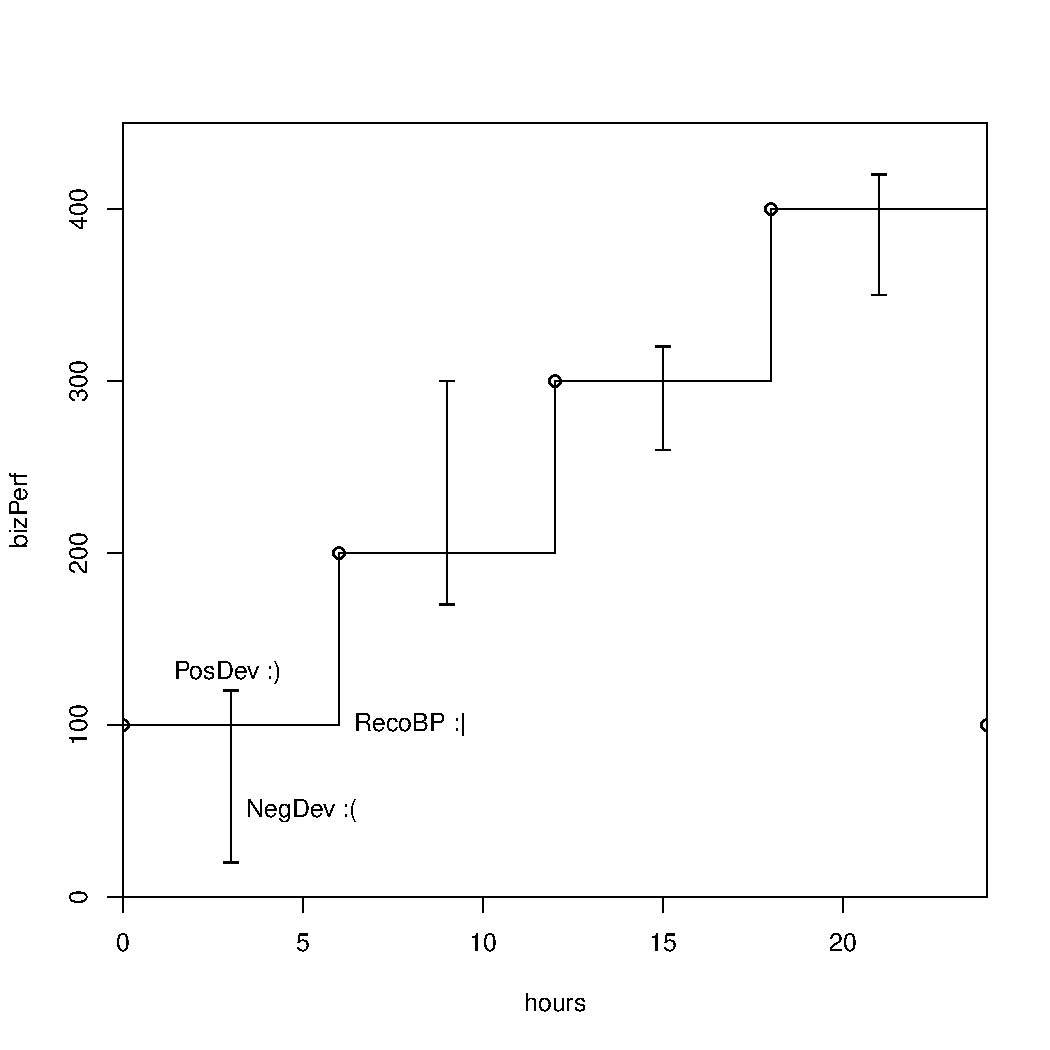
\includegraphics[width=0.99\linewidth]{generated/SFA-candles.pdf}
\caption{Service Flexibility Agreement representation}
\label{fig:SFA}
\end{figure}

\begin{listing}[ht]
\begin{minted} [frame=single, linenos]{yaml}
SFA:
  - Start: 00:00
    End: 06:00
    RecoBP: 100 Hz
    PosDev: 100 Hz/H
    NegDev: 50 Hz/H
  - Start: 07:00
    End: 12:00
    RecoBP: 300 Hz
    PosDev: 50 Hz/H
    NegDev: 200 Hz/H

WorkingModes:
  - WMName: WM1
    actuator: 'cf scale myApp -i 3'
    defaultPower: '300 W'
    maxBusinessPerf: '100 Hz'
  - WMName: WM2
    actuator: 'cf scale myApp -i 5'
    defaultPower: '500 W'
    maxBusinessPerf: '150 Hz'
\end{minted}
\caption{SFA example}
\label{lst:SFA}
\end{listing}

As shown in listing~\ref{lst:SFA} and also represented graphically in figure~\ref{fig:SFA}, for each time frame of a day the SFA defines a recommended business performance (RecoBP, in red in the figure). 
The business performance is one of the KPIs of the application.
For example, for a Web server it is the number of pages served per minutes, for a video transcoding service it will be how many videos can be transcoded per minutes.

We then define a concept called "Happy points", noted "H".
This is an abstraction of the end-user satisfaction.
An application having zero Happy points means that the end user is reasonably satisfied.
An application being allocated exactly the number of resources corresponding to the RecoBP collects 0 Happy points.
This situation corresponds to the traditional SLA threshold.
The positive and negative deviations (PosDev and NegDev) declared in the SFA are then the way that each application "reacts" to being given more or less resources than the RecoBP.
Indeed, some applications such as video transcoding can benefit from receiving temporarily more resources because they can process more videos and thus make their end user happier. 
This kind of application reacts linearly to the amount of resources it is allocated.
On the other hand, an application such as a web server typically have a "turning point" in their relation between performance and resources.
Indeed, giving them less that a certain level of resources (such as the number of front-end VMs) will start to augment the latency in delivering web pages, thus making the end-user unhappy.
On the contrary, giving them more than that level of resources will not have any perceptible impact on the end user, as the latency is already small.
This is represented by the vertical deviation bars in figure~\ref{fig:SFA}: the length of the bar represents the amount of Happy points that the application will win/lose when given more/less performance than the recoBP, respectively.
In this example, at 10 O’clock, if the PaaS framework allocates the resource corresponding to the recommended business performance of 200Hz, the application will collect 0 Happy points.
If the application gets 300Hz, it will get 1H, and one more Happy point for each 100Hz above that.
Conversely, if it gets less than the recommended 200Hz, it will loose Happy point at the rate of one happy point per 25Hz.

We further define the various Working Modes (WM) of an application.
A WM corresponds to a set of resources allocated by the PaaS to an application.
We associate to each WM its typical power consumption and the maximum business performance it can offer.
In practice, a WM corresponds to a number of VMs or Linux Containers, each running instances of the application.
Using the SFA, it is now possible to compute the number of Happy points provided by each WM for each time slot.








\ms{We may refer to a function name like HappyPoints that as input receives performance, and as output gives the number of happy points}

%\ms{I believe more concrete definition is required. We need to establish a better relationship between working mode and SFA. We need better describe working mode and to remove green points.}

%\ms{Or we don't need to refer/define working mode. SFA already corresponds to working mode concept, that is SFA provides various performance levels with different power consumptions}



\section{Collaboration between IaaS and PaaS layers}
\label{sec:iaaspaas}

For this solution to work correctly, an enhanced communication between IaaS and PaaS layers is necessary.
However, this communication should be very carefully designed.
We argue that transmitting too much information between the two layers would be harmful: this would lead to injecting dependencies between the two layers and finally loosing the separation of concerns. \ms{'loosing the separation of concerns' is not clear, need to better define 'the separation of concerns'}

There are essentially two types of information that need to be exchanged, and that will not break the separation of concerns:
\begin{itemize}
  \item VM grouping
  \item VM lifetime
\end{itemize}

We believe that the VM/container grouping is an important information that should be transmitted between the PaaS and the IaaS layers.
Indeed the PaaS layer has a certain degree of knowledge about the applications that are deployed on the cloud.
If an application is composed of several VMs/containers, it would be beneficial to keep them together on the same node, because they will probably have the same life cycle.
Those VMs will probably exchange a lot of information among them. Furthermore, they will probably be switched off together.
This justifies to keep them together on the same node.
Of course, the IaaS layer shouldn't be aware of the applications that are running in the data centre.
However, the VM affinity is an information that could be transmitted to the IaaS when a PaaS manager asks for VM creation.

The other information that is worth transmitting is the VM life-time: an estimated duration that the VM will be kept running before being switched off.
This information is important for the IaaS layer when optimizing the energy consumption of a data centre: indeed to switch off servers it is necessary to migrate VMs. \ms{when consolidation happens, the sentence is not complete and self-sufficient}
However, migrating a VM is an investment, and if the VM is about to be switched off by the PaaS layer, this investment is lost.

Those two informations (VM grouping and VM lifetime) does not break the separation of concerns, because they are expressed in terms of the IaaS VMs only: no deeper knowledge of the running applications is necessary.

\section{Optimization}
\label{sec:optim}

Using the previously described architecture, we can define the optimization to be performed in the data centre. \ms{not sure if we call this architecture, or proposal?}
We define $DC_{Energy}$, the total energy consumption of the data centre, $DC_{Happy}$, the total "happiness" of the data centre and finally $DC_{Brown}$ the consumption of brown energies of the data centre.

\ms{equations are not well defined and well established for energy optimization.}
\begin{equation}
DC_{Energy} =\sum_{time} \sum_{Apps} P_{WMs}
\label{eq:DCen}
\end{equation}

\begin{equation}
DC_{Happy} =\sum_{time} \sum_{Apps} H_{WMs}
\label{eq:DChappy}
\end{equation}

\begin{equation}
DC_{Brown} =\sum_{time} (\sum_{Apps} P_{WMs} \times R_{Brown})
\label{eq:DCbrown}
\end{equation}

The multi-criteria objective followed by the auto-scaler is as the following:

\begin{equation}
\left\{
  \begin{array}{rcr}
    Min & DC_{Energy} \\
    Max & DC_{Happy}  \\
    Min & DC_{Brown}  \\
  \end{array}
\right.
\label{eq:DCbrown}
\end{equation}

\section{Design \& Optimization}
\label{sec:implem}

The SFA is used in the communication between an application and the underlying PaaS framework (while the SLA, on the contrary, is used for the communication between the data centre and its clients), as shown in figure 2.

\begin{figure}[h]
\label{fig:SFABlock}
\centering
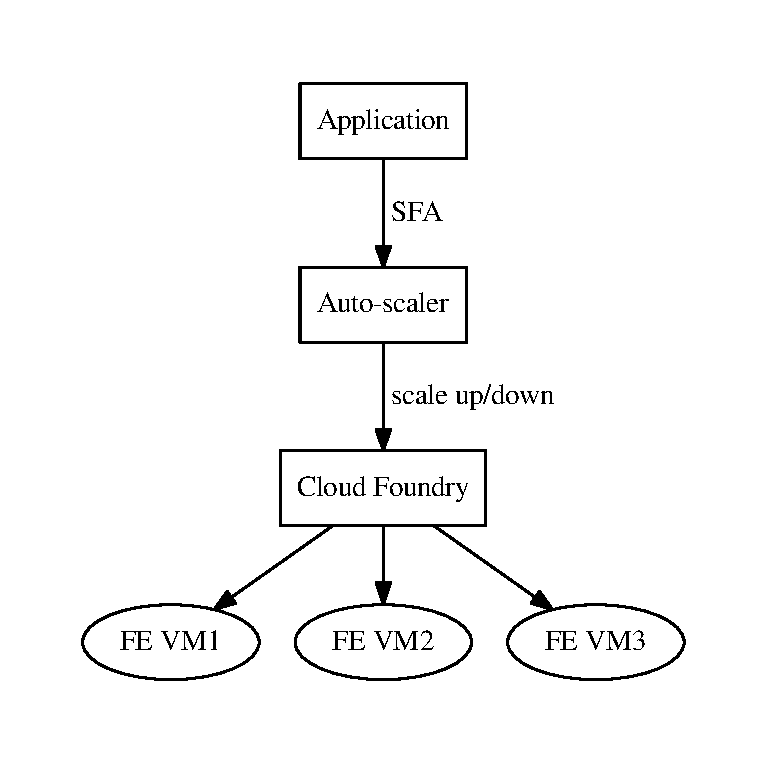
\includegraphics[width=0.6\linewidth]{generated/SFABlock.pdf}
\caption{SFA block diagram}
\end{figure}

In practice, we add a component in the Cloud Foundry stack called the "Optimizer".
This component accepts commands from the application load balancer.
Instead of just scale-up/scale-down commands as it is the case currently, we include a recommended scaling level, together with a positive deviation and a negative deviation, as described in Section~\ref{sec:sfa}.
This will let the Optimizer to optimize according to multiple criteria: 1) the energy consumption in the data centre, 2) the global happiness of the applications (the sum of all happy points granted to applications) and finally 3) the usage of renewable energies.

% !TEX root =  main.tex
\section{Related Works}
\label{sec: relworks}
\cd{in a paper of 4 pages, related works should be very short: I'd say half a page.}
%EE

%IaaS EE
%-VM consolidation %-Scheduling
%History of energy optimization in virtualized datacenters, in a single datacenter
%Workload consolidation is a powerful means to improve IT efficiency and reduce power consumption.
%VM consolidation approaches to reduce energy consumption at IaaS layer have been explored in many recent papers \cite{Cardosa} \cite{ITProf1} \cite{Schroder} \cite{Hermenier2009} \cite{sheikhalishahi_energy_2011} \cite{sheikhalishahi_multi-capacity_2014} \cite{dupont2015plug4green}.

%As a recent development in this field, in \cite{sheikhalishahi_multi-capacity_2014}, authors presented a multi-resource scheduling technique to provide a higher degree of consolidation in multi-dimensional computing systems.

%GreenSLA
%The energy consumption in the data centres depends on several parameters, and it can change according the time and other factors. In order for the environmental impact of data centre energy consumption to be reduced, the data centre must be enabled to respond to energy shaping requests from the energy provider. Therefore, the data centre should have a GreenSLA with the End Users (complementing regular, performance driven service level agreements), including economical and technical parameters in order to realize the contracts effectively, providing discounts or other benefits to the customers meeting and accepting the agreements in order to reduce energy consumption and CO2 emissions, through different policies and strategies

%Therefore, the data centre should have a GreenSLA with the End Users (complementing regular, performance driven service level agreements), including economical and technical parameters in order to realize the contracts effectively, providing discounts or other benefits to the customers meeting and accepting the agreements in order to reduce energy consumption and CO2 emissions, through different policies and strategies
In \cite{botero_greenslas_2013}, GreenSLA is proposed as a flexible SLA to provide levels of performance flexibility in the data center management for reducing energy consumption. GreenSLA requires a close collaboration between the end user and the data center’s energy provider via a contract, providing discounts or other economical benefits to the customers meeting and accepting the agreements in order to reduce energy consumption and CO2 emissions, through different policies and strategies. GreenSLA objectives are economic-incentive to end users in terms of cost-saving, and energy optimization bound to energy provider programs like demand response. In addition, it is very complex requiring contract between end user and data center.

In comparison to GreenSLA, SFA provides more flexibility and opportunity to cloud infrastructure achieving energy efficiency, and resource efficiency objectives in the cloud; while GreenSLA goals are more towards energy and cost. Nonetheless, these two SLA-based approaches are complementary. GreenSLA does not address resource efficiency, whereas SFA does not take into account cost.

\cite{serrano_towards_2013} presents a general framework to address challenges around SLA on the performance, dependability and costs of online cloud services due to ad-hoc management of QoS and SLA. While \cite{serrano_towards_2013} illustrates SLA with QoS metrics such as client request response time, availability, resource usage and resource cost, authors believe that the proposed model and control approach can be applied to other metrics, such as service throughput, and energetic cost. Therefore, research presented in \cite{serrano_towards_2013} is complementary to ours in the sense that it lacks service flexibility definition.

%precisely addresses this issue and makes a threefold contribution. First, it introduces a new cloud model, the SLAaaS (SLA aware Service) model. SLAaaS enables a systematic integration of QoS levels and SLA into the cloud. It is orthogonal to other cloud models such as SaaS or PaaS, and may apply to any of them. Second, the paper introduces CSLA, a novel language to describe QoS-oriented SLA associated with cloud services. Third, the paper presents a control-theoretic approach to provide performance, dependability and cost guarantees for online cloud services, with time-varying workloads. The proposed approach is validated through case studies and extensive experiments with online services hosted in clouds such as Amazon EC2. The case studies illustrate SLA guarantees for various services such as a MapReduce service, a cluster-based multi-tier e-commerce service, and a low-level locking service.

%This paper presents SLA-aware-Service (SLAaaS) cloud model, for a systematic and principled way to integrate quality-of-service (QoS) and service level agreement (SLA) into the cloud. The CSLA specific language is proposed to describe SLAs associated with cloud services in a convenient way. A control-theoretic approach is followed to provide performance, dependability and cost guarantees for online services. Our experiments on online cloud services through various case studies successfully demonstrate the usefulness of SLAaaS.This work opens interesting perspectives in terms of cooperative clouds and cooperative SLAs. We hope that such a model will lead to more principled, less ad-hoc solutions of cloud QoS and SLA management.


%-Scaling operation, Service Flexibility Agreement
In addition, there are energy efficient solutions based on scaling operations (scale up/down application) based on applications performance metrics \cite{vaquero_dynamically_2011}.
Although these proposals reduce the energy footprint of applications and cloud infrastructures, they do not model the applications performance trend to finely define a trade-off between applications Quality of Service and energy footprint.

%Renewable energy availability can estimate a good measure to provide a good consolidation degree.
Autonomic Computing has been exploited in the design of cloud computing architectures in order to devise autonomic loops aiming at providing coordinated actions among cloud layers for efficiency measures, turning each layer of the cloud stack more autonomous, adaptable and aware of the runtime environment \cite{alvares_de_oliveira_synchronization_2012} \cite{de_oliveira_self-management_2012}  \cite{de_oliveira_framework_2013}.

In order to reach a global and efficient state due to conflicting objectives, autonomic loops need to be synchronized.
In \cite{alvares_de_oliveira_synchronization_2012}, authors proposed a generic model to synchronize and coordinate autonomic loops in cloud computing stack. 
The feasibility and scalability of their approach is evaluated via simulation-based experiments on the interaction of several self-adaptive applications with a common self-adaptive infrastructure.


%In \cite{de_oliveira_self-management_2012}, authors propose a self-adaptation approach that considers both application internals and system to reduce the energy footprint in cloud infrastructure. Each application and the infrastructure are equipped with their own control loop, which allows them to autonomously optimize their executions. Simulations show that the approach may lead to appreciable energy savings without interfering on application provider revenues.

In addition to elasticity, scalability is another major advantage introduced by the cloud paradigm.
In \cite{vaquero_dynamically_2011}, automated application scalability in cloud environments are presented.
Authors highlight challenges that will likely be addressed in new research efforts and present an ideal scalable cloud system.

% However, there are some important pending issues before making the dreamed automated scaling for applications come true. 
%We present relevant efforts at the edge of state of the art technology, providing an encompassing overview of the trends they each follow. 

%PaaS-IaaS
\cite{carpen-amarie_towards_2014} proposes a co-design of IaaS and PaaS layers for energy optimization in the cloud. The paper outlines the design of interfaces to enable cross-layer cooperation in clouds. This position paper claims that significant energy gains could be obtained by creating a cooperation API between the IaaS layer and the PaaS layer. Authors discuss two complementary approaches for establishing such cooperation: cross-layer information sharing, and cross-layer coordination.

%PaaS EE
%Containers

%move to INTRO

%Many research efforts have been dedicated to reducing cloud energy consumption, in particular by optimizing the Infrastructure-as-a-Service layer of the Cloud. Infrastructure-as-a-Service (IaaS) is the layer in charge of the virtualization of physical resources, and therefore has direct control over energy-related elements. However, the IaaS layer has no knowledge about the nature of applications which run over these resources, which limits the scope of decisions it can take.
%http://www.conpaas.eu/open-postdoc-position/

%The EcoPaaS project therefore aim at making the IaaS layer (in charge of resources) and the PaaS layer (in charge of applications) collaborate to further reduce the Cloud energy consumption. The idea is to define standard interfaces that allow both layers to exchange relevant information and to coordinate their actions. Exchanging information will for example allow the PaaS layer to estimate the energy consumption of each application it is running. Coordinating actions will in turn allow the system to avoid situations where both layers simultaneously take mutually-damaging actions.

%We will therefore investigate difficult scientific questions such as: which information can and should be exchanged between the two layers? What are the necessary coordination mechanisms to control reconfigurations and avoid detrimental side effects between the two layers? And which energy savings can we potentially obtain if we deployed such techniques in large commercial clouds?

%We will address these questions in the context of the ConPaaS system running over an energy-efficient private cloud such as Snooze. We will follow a systems-oriented methodology based on rigorous experimental data collection, formulation of hypotheses about the necessary mechanisms, prototype implementations, and experimental (in-)validation of the hypotheses.

%In point of fact, from the application provider perspective, Autonomic Computing makes application capable of reacting to a highly variable workload by dynamically adjusting the amount of resources needed to be executed while keeping its Quality of Service (QoS) [11]. From the infrastructure provider point of view, it also makes the infrastructure capable of rapidly reacting to environment changes (e.g. increase/decrease of physical resource usage) by optimizing the allocation of resources and thereby reduce the costs related to energy consumption [4].

%Implementing elasticity to tackle varying workloads while optimizing infrastructures (e.g. utilization rate) and fulfilling applications’ requirements on Quality of Service still remains an open issue and should be addressed by self-adaptation techniques able to manage complexity and dynamism. 

%This model is applied to a Cloud Computing scenario in which several self-adaptive applications interact with a common self-adaptive infrastructure. The objective at the application level is to manage the runtime context to minimize costs while maximizing the QoS, whereas at the infrastructure level, the objective is to manage the context to optimize the utilization rate. 

%Each of the two layers contains information which is potentially relevant for the other in order to reduce the energy footprint of a given application. For example, an energy-aware IaaS may have an estimate of the energy footprint of individual virtual machine types, which may be useful for the PaaS to preferentially select energy-efficient VM instance types. Conversely, a PaaS layer may build short-term traffic predictions which constitute useful hints for IaaS-level consolidation algorithms.

%Both layers should coordinate their reconfiguration actions to reach a state where they help each other in achieving their goals rather than potentially take mutually detrimental decisions. For example, if the IaaS layer decides to migrate a specific VM, then the PaaS could in many cases temporarily reduce the load of the concerned VM to facilitate its migration. Conversely, if the PaaS layer gives early warnings to the IaaS about future requests for creating/destroying resources, the IaaS layer can prepare in advance for these changes. 


%Similarly, [4] proposed an hierarchical autonomic approach for multi-tier web applications. The objective is to deal with several performance and power related problems such as application load balancing, VM consolidation, among others. AMs are categorized according to their overhead on the whole system. For instance, a VM consolidation may involve VM migration and thus should be sparsely performed, whereas the load balancing involves the startup/shutdown of a VM and therefore may be performed more frequently. The interference are managed by sharing the problems’ variables.

%Co-Con [14] is an approach for the coordination of multiple AMs in order to manage power and application-level performance in data centers. It consists of one cluter-level power controller, which adjusts the CPU frequencies of PMs; and several VM-level performance controllers, which adjust the resource fraction allocated the concerned VM based on its actual response time. To avoid interferences, the authors claim that a primary controller (power) must have a control period greater than the settling time of the secondary ones (performance), because hence the secondary ones can achieve a steady state within the control period of the primary one.

%On the one hand, in the context of cloud computing, it is required that managed systems (services) and AMs meet some constraints with respect to information hiding and loose-coupling. On the other hand, AMs which are completely unaware of others managed systems’ context may lead to decisions that impacts negatively services managed by other AMs. The work previously presented do not fit this context due to the high level of details shared among AMs such as application-level performance details or CPU frequencies levels. Instead, this work proposes an event-based coordination mechanism equipped with a public knowledge, which is used by AMs to share a piece of information that can be used within other AMs’ analyses process. The objective is to promote a synergy between AMs while keeping the required level of loose-coupling between AMs.
% !TEX root =  main.tex
\section{Conclusion and Future Work}
\label{sec: conclusion}


\section*{Acknowledgments}

This work has been carried out within the European Projects DC4Cities (FP7-ICT-2013.6.2).

\bibliographystyle{abbrv}
\bibliography{biblio}

\end{document}

%\section{The Energy Adaptive Software Controller}
%
%EASC component provides techniques to shift the workload of running applications in time, to match it with the availability (or forecast availability) of renewable energy.
%The EASC role is to control one application, so as to make it “energy adaptive”, and responsive to the CTRL requests. As such, there should be one EASC configured for each controlled application (as a difference with the DC4ES and CTRL, which are unique in the data centre).
%The EASC plans the activity and control the performance levels of an specific application so as to follow energy budgets provided by the CTRL.
%To enable this, the EASC also has to monitor and predict the energy consumption and activity levels of the application.

%The EASC concepts are sufficiently generic to be applicable to several domains and computing styles within a data centre.
%EASC has been instantiated for batch processing, infrastructure management, web services, and VM management.
%The batch processing EASC manages applications that have typically a fixed amount of work to do during a certain time, such as generating a certain number of reports or applying a virus scan every day.
%On the contrary, the EASC for web services manages applications that must deliver constantly a service, with various levels of performance.
%The infrastructure management EASC covers maintenance operations (such as server decommissioning) performed in an energy efficient way in the data centre.

%Finally, the EASC can also be instantiated to pilot Infrastructure as a Service (IaaS) operations such as anonymous VM resource allocation.

%The EASC allows controlling the software running in data centres in the spatial and the temporal dimensions. As such, there is one EASC per software controlled in the data centre.
%As an input, the EASC receives a list of policies and constraints from the CTRL (the CTRL is described in D3.2).
%As an intermediate output, the EASC will hand back to the CTRL an “option plan”, which is a collection of possible working modes for the application.
%The CTRL will then ask the EASC to apply a selected “activity plan”, which consists of the list of the working modes to apply consecutively.
%Each EASC is then considered as an autonomous system [22] that reacts according to its power budget.
%
%Working Mode
%A working mode corresponds to a level of performance for the controlled application, such as the number of front-end VMs in the case of a web server application.


%\section{cloud transformation}
%We believe DC4C approach is more suitable for existing and future clouds that run a variety of applications. The decentralization of energy adaptive policies to the running software in a data centre allow increasing the possible savings, as the policies can be tweaked to the specific application domain. Furthermore, the central system can make all the EASC collaborate and perform arbitration when needed.
%
%WM:
%Applications can define their working modes based on the following characteristics:
%The number of instances (CF, OS), e.g. WM1 1 instance, WM2 2 instances, etc. Horiz. Scal.
%Resource capacities (CF, OS), e.g. WM1 2 cores, 2GB RAM, etc. Vertical Scal. OS flavor.
%Application Level Scaling: e.g. Parallel Processing: WM1 1 Thread, WM2 2 Processes, etc.
%
%WM optimization:
%OS: Working Modes are encapsulated as VMs.
%It is more efficient to define Wms based on Application Level Scaling, e.g. parallel processing, if possible.
%If we define WM based on resource capacities,  switching WM operation is more costly.
%Resizing operation in OS.
%Or ending a VM, and bring another VM up.
%
%Activity Plan:
%
%Is an ordered list of WMs for timeslots of a timeframe (24hours).
%It is prepared based on renewable energy policies, e.g. aggressive, eager.
%Switching operation happens when moving to a timeslot WM changes respect to the last timeslot.
%
%PaaS architecture in DC4City
%EASC-CFApp1: intermediates between EASC and CF for application App1. It receives activity plan and enact it by invoking CF scaling down/up operations.
%CF is hosted in OS via CF BOSH component.
%PaaS optimization:
%
%IaaS architecture in DC4City
%EASC-OSApp1: intermediates between EASC and OS for application App1. It receives activity plan and enact it by invoking OS resizing operation (Nova API), application level scaling.
%CF is hosted in OS via CF BOSH component.
%IaaS optimization:
